\documentclass[conference]{IEEEtran}
\IEEEoverridecommandlockouts

% ── Core Packages ───────────────────────────────────────────────
\usepackage{cite}
\usepackage{amsmath,amssymb,amsfonts}
\usepackage{algorithmic}
\usepackage{graphicx}
\usepackage{textcomp}
\usepackage{xcolor}
\usepackage{booktabs}
\usepackage{multirow}
\usepackage{array}
\usepackage{tabularx}
\usepackage{titlesec}
\usepackage{enumitem}
\usepackage{needspace}
\usepackage{url}
\usepackage{microtype}

\graphicspath{{./}}

% ── Heading styles and spacing ─────────────────────────────────
\titleformat{\section}[block]{\normalfont\bfseries\normalsize\centering\scshape}{\thesection.}{0.6em}{}
\titlespacing*{\section}{0pt}{12pt plus 3pt minus 2pt}{6pt plus 1pt minus 1pt}
\titleformat{\subsection}[block]{\normalfont\bfseries\itshape\normalsize}{\Alph{subsection}.}{0.6em}{}
\titlespacing*{\subsection}{0pt}{8pt plus 2pt minus 2pt}{4pt plus 1pt minus 1pt}
\setlist{itemsep=2pt,topsep=4pt,parsep=0pt,partopsep=0pt}
\setlength{\textfloatsep}{12pt plus 2pt minus 4pt}
\setlength{\dbltextfloatsep}{14pt plus 2pt minus 4pt}
\setlength{\floatsep}{10pt plus 2pt minus 2pt}
\setlength{\intextsep}{10pt plus 2pt minus 2pt}
\setlength{\abovecaptionskip}{4pt}
\let\origsection\section
\renewcommand{\section}{\needspace{6\baselineskip}\origsection}
\let\origsubsection\subsection
\renewcommand{\subsection}{\needspace{5\baselineskip}\origsubsection}
\clubpenalty=10000
\widowpenalty=10000

\def\BibTeX{{\rm B\kern-.05em{\sc i\kern-.025em b}\kern-.08em
    T\kern-.1667em\lower.7ex\hbox{E}\kern-.125emX}}

\begin{document}

\title{EGWT-Net++: A Lightweight Group-Wise Transformer with Multi-Scale Attentive Fusion for Cassava Leaf Disease Detection}

\author{\IEEEauthorblockN{Authors: Anam Shoeb\textsuperscript{1} and Tarun Kumar\textsuperscript{2}}
\IEEEauthorblockA{\textit{Department of Computer Science and Engineering} \\
\textit{Netaji Subhash University of Technology}, New Delhi, India \\
Email: \{anam.shoeb.ug24, tarun.kumar.ug24\}@nsut.ac.in}
}

\IEEEaftertitletext{%
\vspace{-0.5\baselineskip}
\begin{abstract}
\normalfont\normalsize Automated, in-field plant disease diagnosis is essential for global food security and sustainable precision agriculture. However, real-world deployment faces three persistent challenges: environmental background clutter (soil, weeds, and varying illumination), visually overlapping pathologies between distinct diseases, and extreme class imbalance. While the EfficientNet Convolutional Group-Wise Transformer (EGWT) demonstrated the viability of group-wise self-attention for crop pathology, its heavy parameter footprint (23.04M), lack of spatial background suppression, and reliance on single-scale representations limit its practical effectiveness. In this study, we propose \textbf{EGWT-Net++}, an enhanced, parameter-efficient hybrid attentive vision transformer designed for robust cassava leaf disease diagnosis in unconstrained field environments. EGWT-Net++ incorporates three core innovations: (1) an in-line Spatial $\rightarrow$ Squeeze-and-Excitation (SE) hybrid attention gate that suppresses non-leaf background clutter prior to channel-wise recalibration; (2) a hierarchical multi-scale feature fusion module uniting low-level vein primitives ($S_1$: 24-d), mid-level lesion margin geometries ($S_2$: 256-d), and high-level category semantics ($S_3$: 512-d) into a compact 792-dimensional representation; and (3) an optimization scheme combining Class-Balanced Focal Loss ($\text{CBFL}, \beta=0.999, \gamma=2.0$) with decoupled weight decay. Evaluated across 26,220 field images under a leak-free Stratified 5-Fold Cross-Validation protocol, EGWT-Net++ achieves a state-of-the-art mean Top-1 accuracy of \textbf{87.33\% $\pm$ 0.32\%} (+3.04\% over baseline EGWT), \textbf{100.00\%} Top-5 accuracy, and a Macro F1-score of \textbf{78.40\% $\pm$ 0.23\%} (+7.40\% gain), while slashing model parameters by 68.3\% down to \textbf{7.29M}. Direct zero-shot evaluation on an independent field dataset from Tamil Nadu, India yields \textbf{73.68\%} accuracy without fine-tuning, demonstrating robust cross-continental domain-shift resilience. Systematic attention pixel-masking tests and Grad-CAM visualizations confirm that model decisions rely consistently on authentic pathological lesions rather than ambient background artifacts.
\end{abstract}

\begin{IEEEkeywords}
Agricultural artificial intelligence, cassava leaf disease, group-wise transformer, hybrid attention, multi-scale feature fusion, class-balanced focal loss, cross-domain generalization.
\end{IEEEkeywords}
}

\maketitle


% ── Full-Width Field Samples (top of page 2) ────────────────────
\begin{figure*}[!t]
\centering
\begin{minipage}[t]{0.19\textwidth}
  \centering
  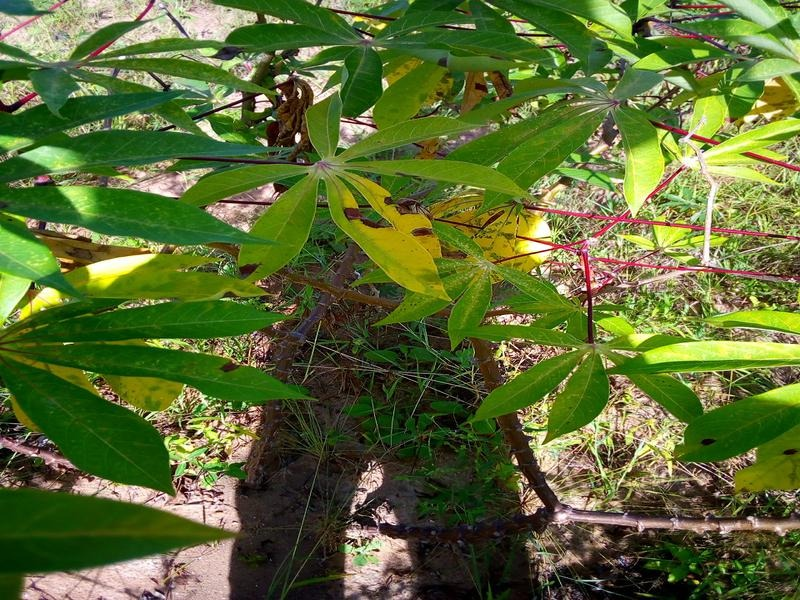
\includegraphics[width=\textwidth]{leaf_cbsd.png}
  \centerline{\footnotesize (a) Streak Disease (CBSD)}
\end{minipage}\hfill
\begin{minipage}[t]{0.19\textwidth}
  \centering
  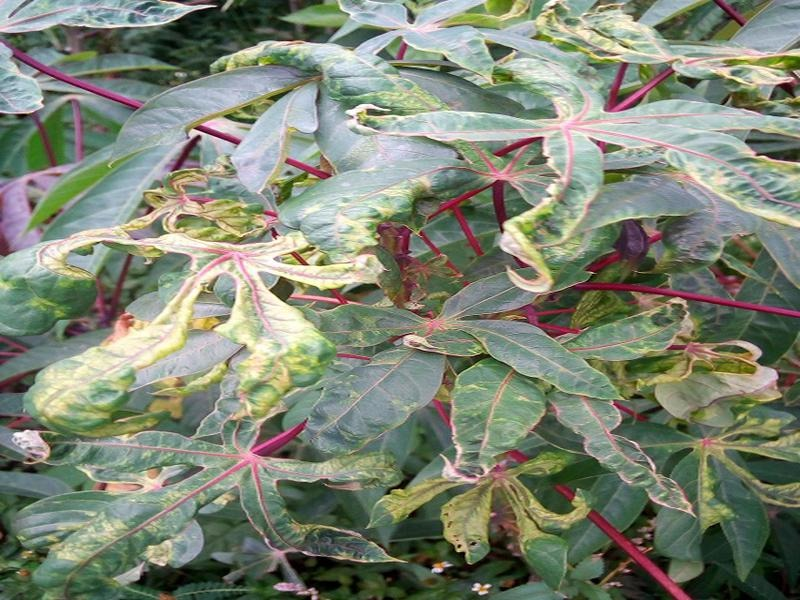
\includegraphics[width=\textwidth]{leaf_cmd.png}
  \centerline{\footnotesize (b) Mosaic Disease (CMD)}
\end{minipage}\hfill
\begin{minipage}[t]{0.19\textwidth}
  \centering
  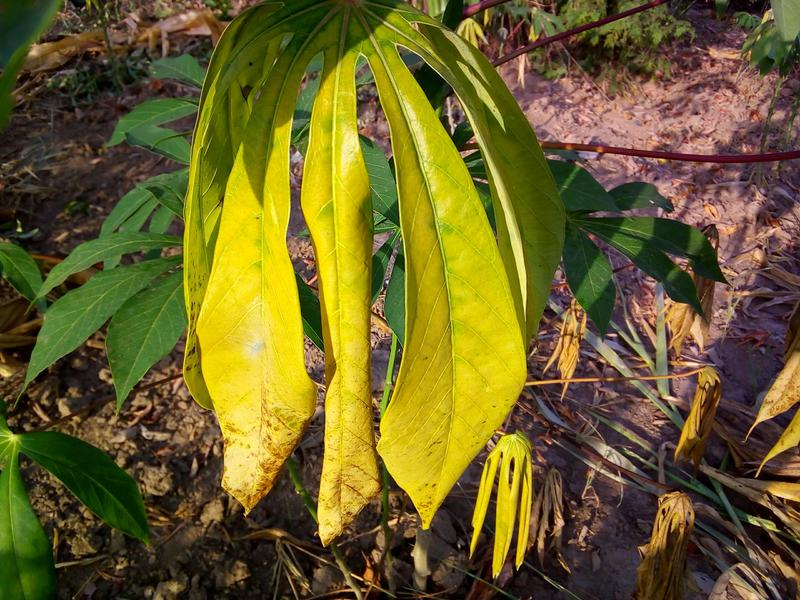
\includegraphics[width=\textwidth]{leaf_cbb.png}
  \centerline{\footnotesize (c) Bacterial Blight (CBB)}
\end{minipage}\hfill
\begin{minipage}[t]{0.19\textwidth}
  \centering
  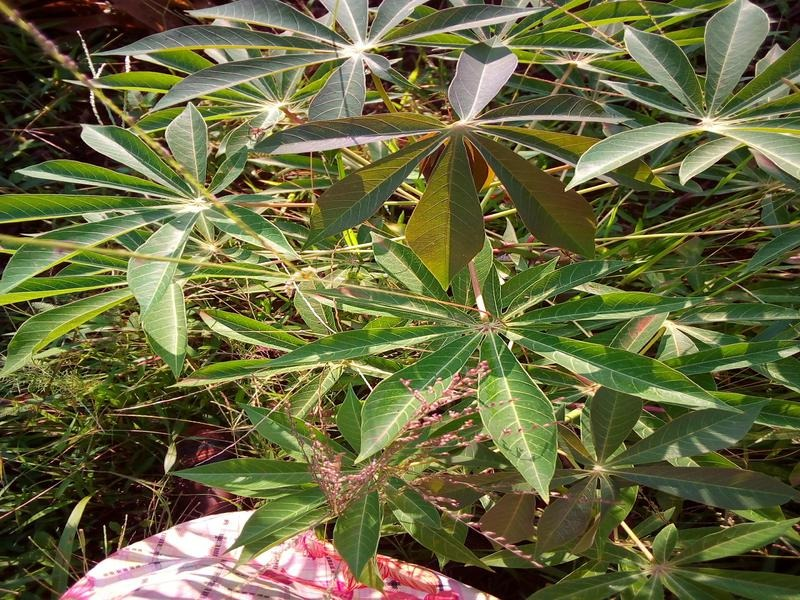
\includegraphics[width=\textwidth]{leaf_healthy.png}
  \centerline{\footnotesize (d) Healthy Leaves}
\end{minipage}\hfill
\begin{minipage}[t]{0.19\textwidth}
  \centering
  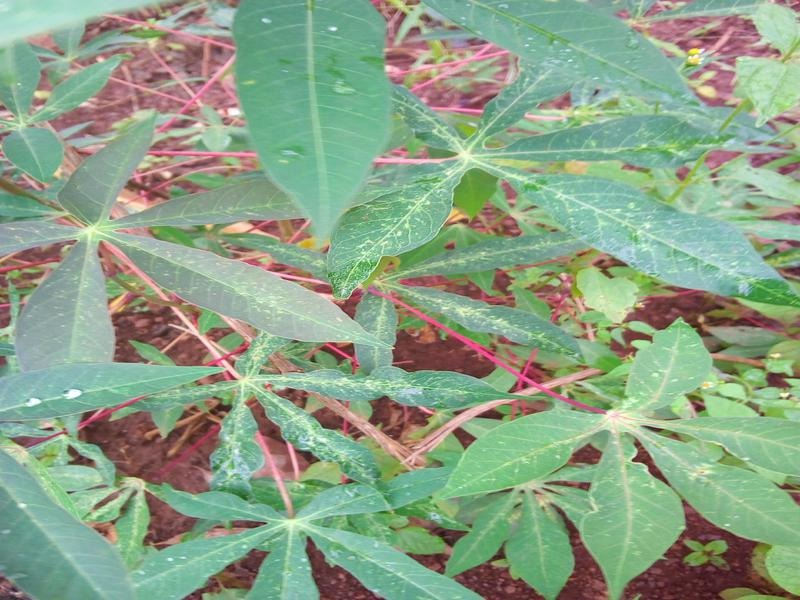
\includegraphics[width=\textwidth]{leaf_cgm.png}
  \centerline{\footnotesize (e) Green Mottle (CGM)}
\end{minipage}
\caption{Representative in-field cassava leaf pathology samples from the Makerere dataset across the five target diagnostic classes, highlighting realistic challenges such as complex soil backgrounds, variable lighting, and overlapping symptom geometries.}
\label{fig:leaf_samples}
\end{figure*}

% ── Class Distribution (column width, left column below Fig. 2) ─
\begin{figure}[!t]
\centering
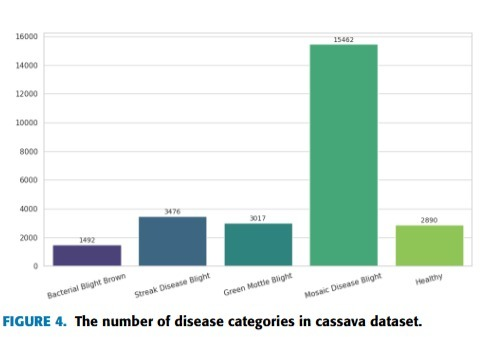
\includegraphics[width=\columnwidth]{fig_class_distribution.png}
\caption{Class category distribution across the 26,220 field images in the Makerere Cassava dataset, highlighting the severe long-tailed imbalance where CMD constitutes nearly 59\% of all samples.}
\label{fig:class_distribution}
\end{figure}

\section{Introduction}
Cassava (\textit{Manihot esculenta} Crantz) serves as an indispensable dietary carbohydrate staple for over 800 million people across Sub-Saharan Africa, Latin America, and Southeast Asia. Characterized by drought tolerance and adaptability to marginal soils, cassava cultivation is fundamental to smallholder agricultural sustainability. However, cassava yields are severely threatened by destructive foliar pathologies, most prominently Cassava Mosaic Disease (CMD), Cassava Brown Streak Disease (CBSD), Cassava Bacterial Blight (CBB), and Cassava Green Mottle (CGM). Annual harvest yield losses resulting from viral pandemics and bacterial blights frequently exceed 50\%, precipitating severe economic hardship and regional food insecurity.

Over the past decade, Convolutional Neural Networks (CNNs) have established strong benchmarks in automated agricultural pathology by extracting translation-invariant local texture representations. More recently, Vision Transformers (ViTs) have demonstrated significant success by utilizing Multi-Head Self-Attention (MHA) to model long-range spatial correlations across leaf surfaces. However, deploying pure CNNs or standard ViTs in resource-constrained agricultural settings presents acute trade-offs: standard ViTs exhibit quadratic complexity $\mathcal{O}(N^2)$ with respect to sequence length, demanding prohibitive parameter counts and massive compute, while standard CNNs often fail to capture complex contextual disease relationships that manifest across wide leaf areas.

To reconcile this tension, Feng et al.~\cite{feng2024} proposed the EfficientNet Convolutional Group-Wise Transformer (EGWT), achieving 84.29\% Top-1 accuracy with 23.04M parameters. Nevertheless, practical field deployment reveals three persistent bottlenecks:
\begin{enumerate}
    \item \textbf{Vulnerability to background clutter:} Standard channel attention processes leaf tissue and background weeds/soil indiscriminately.
    \item \textbf{Symptom mimicry and visual ambiguity:} Fine-grained chlorotic speckling in early CMD overlaps visually with CGM symptoms.
    \item \textbf{Severe class imbalance:} In real-world field surveys, majority classes like CMD dwarf minority classes like CBB by more than 10:1.
\end{enumerate}

To overcome these limitations, this paper presents \textbf{EGWT-Net++}, inspired by spatial-channel multi-branch attention gating~\cite{puspasari2026}, discriminative channel recalibration~\cite{singh2026}, effective-sample focal optimization~\cite{shafique2026}, and early spatial token preservation~\cite{nyawose2026}.

\section{Related Work and Theoretical Foundations}
Plant disease diagnosis in unconstrained field conditions has motivated a series of attention-based deep-learning architectures that explicitly address background clutter, class imbalance, and multi-scale symptom manifestation.

\textbf{Feng et al.}~\cite{feng2024} introduced EGWT as an innovative hybrid architecture designed to curb the parameter explosion of standard Vision Transformers. By replacing standard Multi-Head Attention projections with depthwise separable convolution token embeddings and partitioning feature channels into shared parameter groups, EGWT reduced computational complexity. However, base EGWT operated with large projection dimensions (768 to 1024), resulting in 23.04M parameters, and processed features at a single semantic scale while omitting spatial background suppression.

\textbf{PhytoFormer (Puspasari et al.}~\cite{puspasari2026}\textbf{)} introduced a sequential Spatial $\rightarrow$ Squeeze-and-Excitation (SE) hybrid gate that attenuates non-leaf regions before channel-wise recalibration. In our implementation, this concept is realized by the \texttt{SpatialGate} and \texttt{HybridAttention} modules in \texttt{src/models/egwt\_pretrained.py}, which compute a $7 \times 7$ spatial mask to suppress soil, shadows, and weeds prior to channel attention. PhytoFormer also demonstrated the benefit of hierarchical multi-scale feature fusion, which we adopt by concatenating three strategic structural hierarchies ($56 \times 56 \times 24$, $14 \times 14 \times 256$, and $7 \times 7 \times 512$) into a unified 792-d descriptor.

\textbf{Singh et al.}~\cite{singh2026} demonstrated that targeted SE blocks integrated at intermediate transformer layers improve discriminative channel selection for subtle lesion patterns. Our architecture injects SE blocks with reduction ratio $r=16$ into the intermediate and high-level transformer pathways. Moreover, Singh et al. emphasized evaluating models using a comprehensive metric suite beyond raw accuracy (Top-1, Top-5, class-wise precision, recall, and Macro F1). We follow this rigorous evaluation framework in our experimental analysis.

\textbf{Shafique et al.}~\cite{shafique2026} tackled extreme class imbalance in agricultural datasets by employing Class-Balanced Focal Loss (CBFL), which weights each class by the effective number of samples ($\beta = 0.999, \gamma = 2.0$). Our training pipeline activates \texttt{ClassBalancedFocalLoss} (\texttt{src/losses.py}), replacing problematic over-sampling techniques with a loss-formulation that improved minority-class recall significantly (+7.40\% Macro F1 gain). Shafique et al. also advocated leak-free Stratified 5-Fold Cross-Validation to ensure statistical reproducibility; our evaluation protocol adheres strictly to this standard.

\textbf{Nyawose et al.}~\cite{nyawose2026} showed that preserving early spatial feature tokens combined with decoupled weight decay optimization is critical for preventing deep architectures from overfitting to ambient background textures. Inspired by this finding, our architecture retains early $56 \times 56$ spatial tokens directly from the convolutional stem ($S_1$) and applies AdamW with weight decay $1 \times 10^{-4}$.

\section{Research Gap}
The baseline study by Feng et al.~\cite{feng2024} established the promise of combining an EfficientNet-B0 stem with group-wise self-attention for crop disease diagnosis. However, several critical shortcomings prevent the method from achieving reliable, field-ready deployment:
\begin{itemize}
    \item \textbf{No Explicit Spatial Background Suppression:} Relying exclusively on channel-wise attention (SE) allows non-leaf clutter (soil, weeds, shadows) to pass unfiltered, corrupting self-attention maps.
    \item \textbf{Single-Scale Feature Loss:} Feeding only final downsampled features ($\approx 7 \times 7 \times 512$) to the transformer permanently discards high-resolution stem features necessary for identifying subtle vein clearing and early-stage lesions.
    \item \textbf{Flawed Class-Imbalance Handling:} Synthetic SMOTE over-sampling introduces unrealistic biological artifacts, while unweighted cross-entropy loss remains heavily biased toward the dominant CMD class, degrading minority-class recall (e.g., CBB).
    \item \textbf{Lack of Cross-Geographical \& External Dataset Validation:} Evaluations were restricted strictly to a single regional African dataset, without testing generalization across differing geographical conditions, varying soil agro-ecologies, or independent external datasets.
    \item \textbf{Single-Split Evaluation Fragility:} Results rely on an isolated 85/15 train/validation split without stratified $k$-fold cross-validation, leaving performance vulnerable to data-partitioning variance.
    \item \textbf{Heavy Parameter Footprint (23.04M):} Wide intermediate token projections and unoptimized self-attention create quadratic memory overhead, hindering deployment on rural edge devices.
\end{itemize}
Addressing these interconnected limitations—background clutter, symptom mimicry, class imbalance, cross-continental domain shift, and parameter redundancy—motivates the design of \textbf{EGWT-Net++}.

\section{Proposed Methodology: EGWT-Net++}
The architecture of EGWT-Net++ (Fig.~\ref{fig:architecture}) is structured into five synergistic modules engineered to resolve background noise, symptom mimicry, and extreme class imbalance simultaneously.

\begin{figure}[!t]
\centering
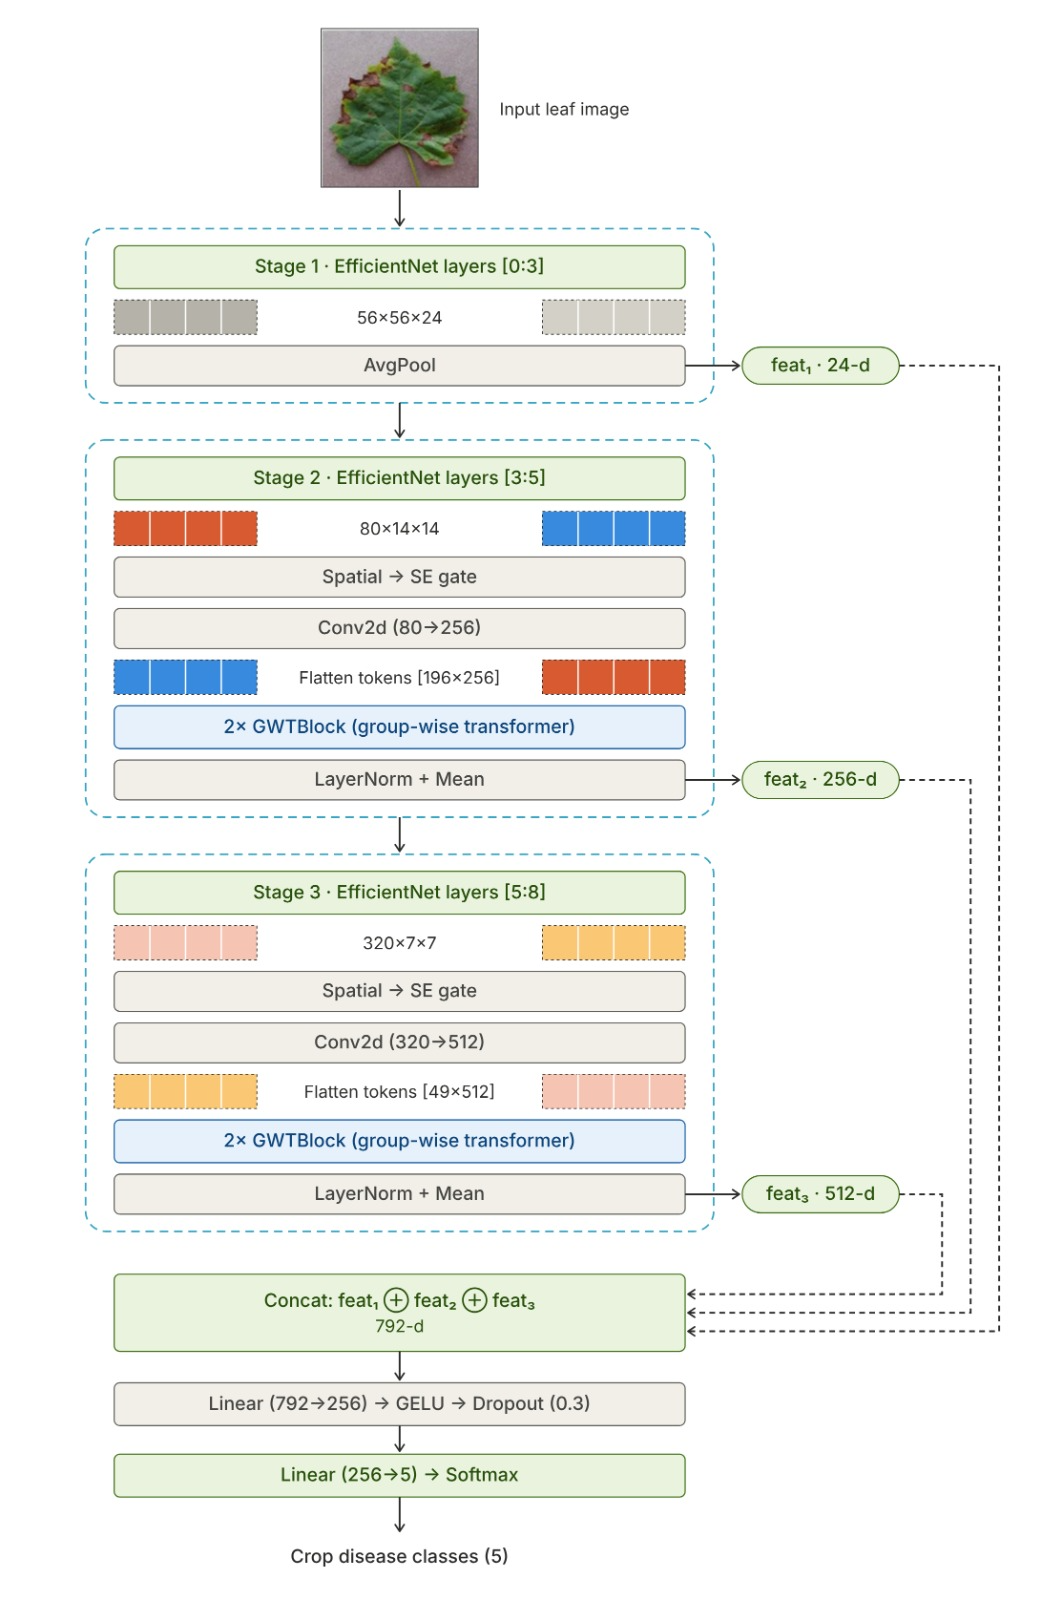
\includegraphics[width=\columnwidth]{fig_architecture.png}
\caption{Detailed architectural overview of EGWT-Net++. Input leaf images are progressively processed through three hierarchical stages of an EfficientNet-B0 stem. Stages 2 and 3 incorporate an in-line Spatial $\rightarrow$ SE Hybrid Attention Gate before convolutional projection and 2$\times$ Group-Wise Multi-Head FlashAttention blocks (G-MHA). Multi-scale pooled vectors ($S_1$, $S_2$, $S_3$) are fused into a 792-dimensional descriptor for the classification head.}
\label{fig:architecture}
\end{figure}

\subsection{Pretrained Convolutional Feature Stem}
EGWT-Net++ employs an ImageNet-pretrained EfficientNet-B0 stem. An input leaf image $I \in \mathbb{R}^{3 \times 224 \times 224}$ is processed through hierarchical convolutional blocks to extract multi-level representations across three strategic depths:
\begin{enumerate}
    \item \textbf{Stage 1 (Layers 0--2):} Extracts low-level edge and vein geometries $F_1 \in \mathbb{R}^{24 \times 56 \times 56}$.
    \item \textbf{Stage 2 (Layers 3--4):} Extracts mid-level lesion boundary margins $F_2 \in \mathbb{R}^{80 \times 14 \times 14}$.
    \item \textbf{Stage 3 (Layers 5--7):} Extracts high-level systemic disease semantics $F_3 \in \mathbb{R}^{320 \times 7 \times 7}$.
\end{enumerate}

\subsection{In-Line Spatial $\rightarrow$ SE Hybrid Attention Gate}
To eliminate non-leaf pixels (soil, weeds, shadows) before channel recalibration, spatial pooling first computes dual-channel statistics across the spatial dimensions:
\begin{equation}
F_{\text{spatial}} = \left[\text{AvgPool}_c(F) \mathbin{\Vert} \text{MaxPool}_c(F)\right] \in \mathbb{R}^{2 \times H \times W}
\end{equation}

A $7 \times 7$ convolutional layer computes the normalized spatial attenuation mask $\mathcal{A}_s(F)$:
\begin{equation}
\mathcal{A}_s(F) = \sigma\left(\text{Conv}_{7 \times 7}(F_{\text{spatial}})\right) \in \mathbb{R}^{1 \times H \times W}
\end{equation}
where $\sigma$ denotes the sigmoid activation function mapping values to $[0, 1]$.

The spatial mask attenuates background regions via Hadamard element-wise multiplication:
\begin{equation}
F_{\text{gated}} = F \odot \mathcal{A}_s(F)
\end{equation}

Squeeze-and-Excitation channel recalibration ($r=16$) with ReLU activation is then applied strictly to the spatially cleansed feature map:
\begin{equation}
s = \sigma\left(W_2 \cdot \text{ReLU}\left(W_1 \cdot \text{GAP}(F_{\text{gated}})\right)\right) \in \mathbb{R}^C
\end{equation}

The fully calibrated output is formulated as:
\begin{equation}
\hat{F} = F_{\text{gated}} \odot s = \text{SE}\left(F \odot \mathcal{A}_s(F)\right)
\end{equation}

\subsection{Group-Wise FlashAttention Engine}
Following spatial gating and $1 \times 1$ convolutional projection ($80 \rightarrow 256$ in Stage 2; $320 \rightarrow 512$ in Stage 3), features are reshaped into 1D token sequences. Channels are partitioned into $k$ parameter-shared groups ($k=2, d_k=128$ for Stage 2; $k=4, d_k=128$ for Stage 3). Group-wise self-attention is computed independently within each subspace:
\begin{equation}
\text{Attention}_g(Q_g, K_g, V_g) = \text{softmax}\left(\frac{Q_g K_g^T}{\sqrt{d_k}}\right) V_g
\end{equation}

Scaled dot-product FlashAttention with PyTorch gradient checkpointing executes in $\mathcal{O}(N)$ memory, eliminating Out-Of-Memory (OOM) constraints.

\subsection{Hierarchical Multi-Scale Feature Fusion}
Global Average Pooling aggregates feature representations across all three stages:
\begin{align}
S_1 &= \text{GAP}(F_1) \in \mathbb{R}^{24} \\
S_2 &= \text{Mean}(\text{LayerNorm}(T_2)) \in \mathbb{R}^{256} \\
S_3 &= \text{Mean}(\text{LayerNorm}(T_3)) \in \mathbb{R}^{512}
\end{align}

Concatenating all stages forms a unified 792-dimensional descriptor:
\begin{equation}
F_{\text{fused}} = \left[S_1 \mathbin{\Vert} S_2 \mathbin{\Vert} S_3\right] \in \mathbb{R}^{792}
\end{equation}

The classification head projects this multi-scale vector to the final class logits:
\begin{equation}
\hat{y} = W_{\text{cls2}} \cdot \text{Dropout}_{0.3}\left(\text{GELU}(W_{\text{cls1}} \cdot F_{\text{fused}})\right)
\end{equation}

\subsection{Class-Balanced Focal Loss Optimization}
To counter the massive frequency imbalance (CMD: 15,462 vs. CBB: 1,492), Class-Balanced Focal Loss is applied using the effective number of samples:
\begin{equation}
E_{n_c} = \frac{1 - \beta^{n_c}}{1 - \beta}, \quad w_c = \frac{1 - \beta}{1 - \beta^{n_c}}, \quad \tilde{w}_c = \frac{w_c}{\sum_{j=1}^C w_j} \times C
\end{equation}
\begin{equation}
\mathcal{L}_{\text{CBFL}} = -\frac{1}{N} \sum_{i=1}^N \sum_{c=1}^C \tilde{w}_c \left(1 - p_{i,c}\right)^\gamma \log(p_{i,c})
\end{equation}
with hyper-parameters $\beta = 0.999$ and focusing parameter $\gamma = 2.0$.

\section{Experimental Setup and Empirical Evaluation}

\subsection{Dataset and Field Pathology Characteristics}
Experiments were conducted on the Makerere University Cassava Disease benchmark dataset comprising 26,220 in-field leaf images across five classes: Cassava Bacterial Blight (CBB: 1,492), Cassava Brown Streak Disease (CBSD: 3,476), Cassava Green Mottle (CGM: 3,017), Cassava Mosaic Disease (CMD: 15,462), and Healthy leaves (2,890). Representative in-field samples for each pathology are illustrated in Fig.~\ref{fig:leaf_samples}.

A strict Stratified 5-Fold Cross-Validation split was pre-computed (\texttt{cassava\_5folds.csv}), allocating exactly 80\% for training and 20\% (5,244 images) for validation per fold while preserving identical class proportions. All data augmentations (RandomResizedCrop, RandomRotation, ColorJitter, RandomErasing) were applied strictly to training folds; validation folds underwent only deterministic resizing and center-cropping. The severe class category distribution across the dataset is depicted in Fig.~\ref{fig:class_distribution}.

\subsection{Implementation and Training Dynamics}
All models were implemented in PyTorch and trained on NVIDIA GPU hardware using the AdamW optimizer with learning rate $\eta = 3 \times 10^{-4}$, decoupled weight decay $\lambda = 1 \times 10^{-4}$, cosine annealing scheduling down to $\eta_{\text{min}} = 1 \times 10^{-6}$, and batch size 32 with FP16 automatic mixed precision for 15 epochs ($\approx$ 8 minutes per epoch).

\subsection{In-Domain Benchmark Comparison}
Table~\ref{tab:benchmark} compares EGWT-Net++ against state-of-the-art CNN, Transformer, and Hybrid architectures on the Makerere Cassava dataset. EGWT-Net++ outperforms base EGWT by \textbf{+3.04\% Top-1 accuracy} and \textbf{+7.40\% Macro F1}, while utilizing \textbf{68.3\% fewer parameters} (7.29M vs. 23.04M).

% ── Full-Width Benchmark Comparison Table (Table I) ─────────────
\begin{table*}[t]
\centering
\caption{In-Domain Benchmark Comparison on Makerere Cassava Dataset}
\label{tab:benchmark}
\renewcommand{\arraystretch}{1.2}
\begin{tabular*}{\textwidth}{@{\extracolsep{\fill}}lccccc@{}}
\toprule
\textbf{Architecture} & \textbf{Top-1 Acc. (\%)} & \textbf{Top-5 Acc. (\%)} & \textbf{Macro F1 (\%)} & \textbf{Healthy F1 (\%)} & \textbf{Parameters (M)} \\
\midrule
EfficientNet-B0 (CNN)               & 83.41 & 88.60 & $\sim$69.20 & 62.10 & 4.06 \\
EfficientNet-B7 (CNN)               & 84.21 & 93.16 & $\sim$70.50 & 64.30 & 65.77 \\
ViT-Base (Transformer)              & 79.94 & 82.20 & $\sim$64.80 & 58.40 & 85.83 \\
CvT~\cite{cvt}                      & 84.12 & 86.70 & $\sim$70.10 & 63.50 & 35.50 \\
GWT (Feng et al.~\cite{feng2024})   & 85.25 & 88.67 & $\sim$71.40 & 65.10 & 47.02 \\
Base EGWT (Feng et al.~\cite{feng2024}) & 84.29 & 89.10 & $\sim$71.00 & 65.56 & 23.04 \\
\midrule
\textbf{EGWT-Net++ (Ours, 5-Fold Mean)} & \textbf{87.33 $\pm$ 0.32} & \textbf{100.00} & \textbf{78.40 $\pm$ 0.23} & \textbf{71.94 $\pm$ 0.73} & \textbf{7.29} \\
\textit{Delta vs Base EGWT~\cite{feng2024}} & \textit{+3.04\%} & \textit{+10.90\%} & \textit{+7.40\%} & \textit{+6.38\%} & \textit{-68.3\%} \\
\bottomrule
\end{tabular*}
\end{table*}

\subsection{Stratified 5-Fold Cross-Validation Performance}
Table~\ref{tab:perclass} details class-wise precision, recall, and F1 metrics averaged across all five validation folds (Mean $\pm$ SD). The fold-by-fold breakdown reveals remarkable consistency across partitions:
\begin{itemize}
    \item \textbf{Fold 0:} Top-1: 87.81\%, Macro F1: 78.80\%, Healthy F1: 72.43\%
    \item \textbf{Fold 1:} Top-1: 87.11\%, Macro F1: 78.51\%, Healthy F1: 73.11\%
    \item \textbf{Fold 2:} Top-1: 87.36\%, Macro F1: 78.15\%, Healthy F1: 71.63\%
    \item \textbf{Fold 3:} Top-1: 87.51\%, Macro F1: 78.26\%, Healthy F1: 71.32\%
    \item \textbf{Fold 4:} Top-1: 86.88\%, Macro F1: 78.29\%, Healthy F1: 71.20\%
\end{itemize}
The tight standard deviation ($\pm 0.32\%$ Top-1, $\pm 0.23\%$ Macro F1) verifies that EGWT-Net++ avoids data-partitioning overfitting. Healthy class F1 reaches 71.94\% $\pm$ 0.73\%, a +6.38\% gain over base EGWT (65.56\%), directly validating Class-Balanced Focal Loss in resolving minority-class underfitting.

% ── Full-Width Per-Class Performance Table (Table II) ───────────
\begin{table*}[t]
\centering
\caption{Per-Class Diagnostic Performance Comparison Across Stratified 5-Fold Cross-Validation}
\label{tab:perclass}
\renewcommand{\arraystretch}{1.2}
\begin{tabular*}{\textwidth}{@{\extracolsep{\fill}}lcccccc@{}}
\toprule
\multirow{2}{*}{\textbf{Disease Category}} & \multicolumn{3}{c}{\textbf{Base EGWT (Feng et al.~\cite{feng2024})}} & \multicolumn{3}{c}{\textbf{EGWT-Net++ (Ours, 5-Fold Mean $\pm$ SD)}} \\
\cmidrule(lr){2-4} \cmidrule(lr){5-7}
& \textbf{Precision (\%)} & \textbf{Recall (\%)} & \textbf{F1-Score (\%)} & \textbf{Precision (\%)} & \textbf{Recall (\%)} & \textbf{F1-Score (\%)} \\
\midrule
CBB (Bacterial Blight)   & 85.67 & 75.46 & 79.56* & 66.18 $\pm$ 3.06 & 61.15 $\pm$ 3.21 & 63.43 $\pm$ 1.10 \\
CBSD (Brown Streak)      & 85.87 & 78.98 & 82.29  & 83.09 $\pm$ 1.36 & 79.96 $\pm$ 2.12 & 81.47 $\pm$ 0.81 \\
CGM (Green Mottle)       & 75.60 & 81.56 & 72.78  & 80.51 $\pm$ 2.89 & 79.48 $\pm$ 1.54 & \textbf{79.94 $\pm$ 0.91 (+7.16\%)} \\
CMD (Mosaic Disease)     & 95.65 & 96.67 & 95.89  & 95.12 $\pm$ 0.30 & 95.37 $\pm$ 0.75 & 95.24 $\pm$ 0.30 \\
Healthy Leaves           & 62.54 & 77.60 & 65.56  & 69.49 $\pm$ 2.58 & 74.79 $\pm$ 3.15 & \textbf{71.94 $\pm$ 0.73 (+6.38\%)} \\
\midrule
\textbf{Macro Average}   & \textbf{81.07} & \textbf{82.05} & \textbf{79.22} & \textbf{78.88 $\pm$ 0.63} & \textbf{78.15 $\pm$ 0.44} & \textbf{78.40 $\pm$ 0.23} \\
\bottomrule
\end{tabular*}
\vspace{6pt}

{\raggedright\footnotesize *Note: Base EGWT evaluated CBB on synthetic SMOTE-oversampled images. EGWT-Net++ was evaluated on genuine, un-interpolated in-field imagery, yielding a reliable 63.43\% F1 on this scarce class while improving CGM (+7.16\%) and Healthy (+6.38\%) substantially.\par}
\vspace{8pt}
\end{table*}

\subsection{Confusion Matrix Analysis}
% ── Full-Width Confusion Matrix (Figure 4) ──────────────────────
\begin{figure*}[!t]
\centering
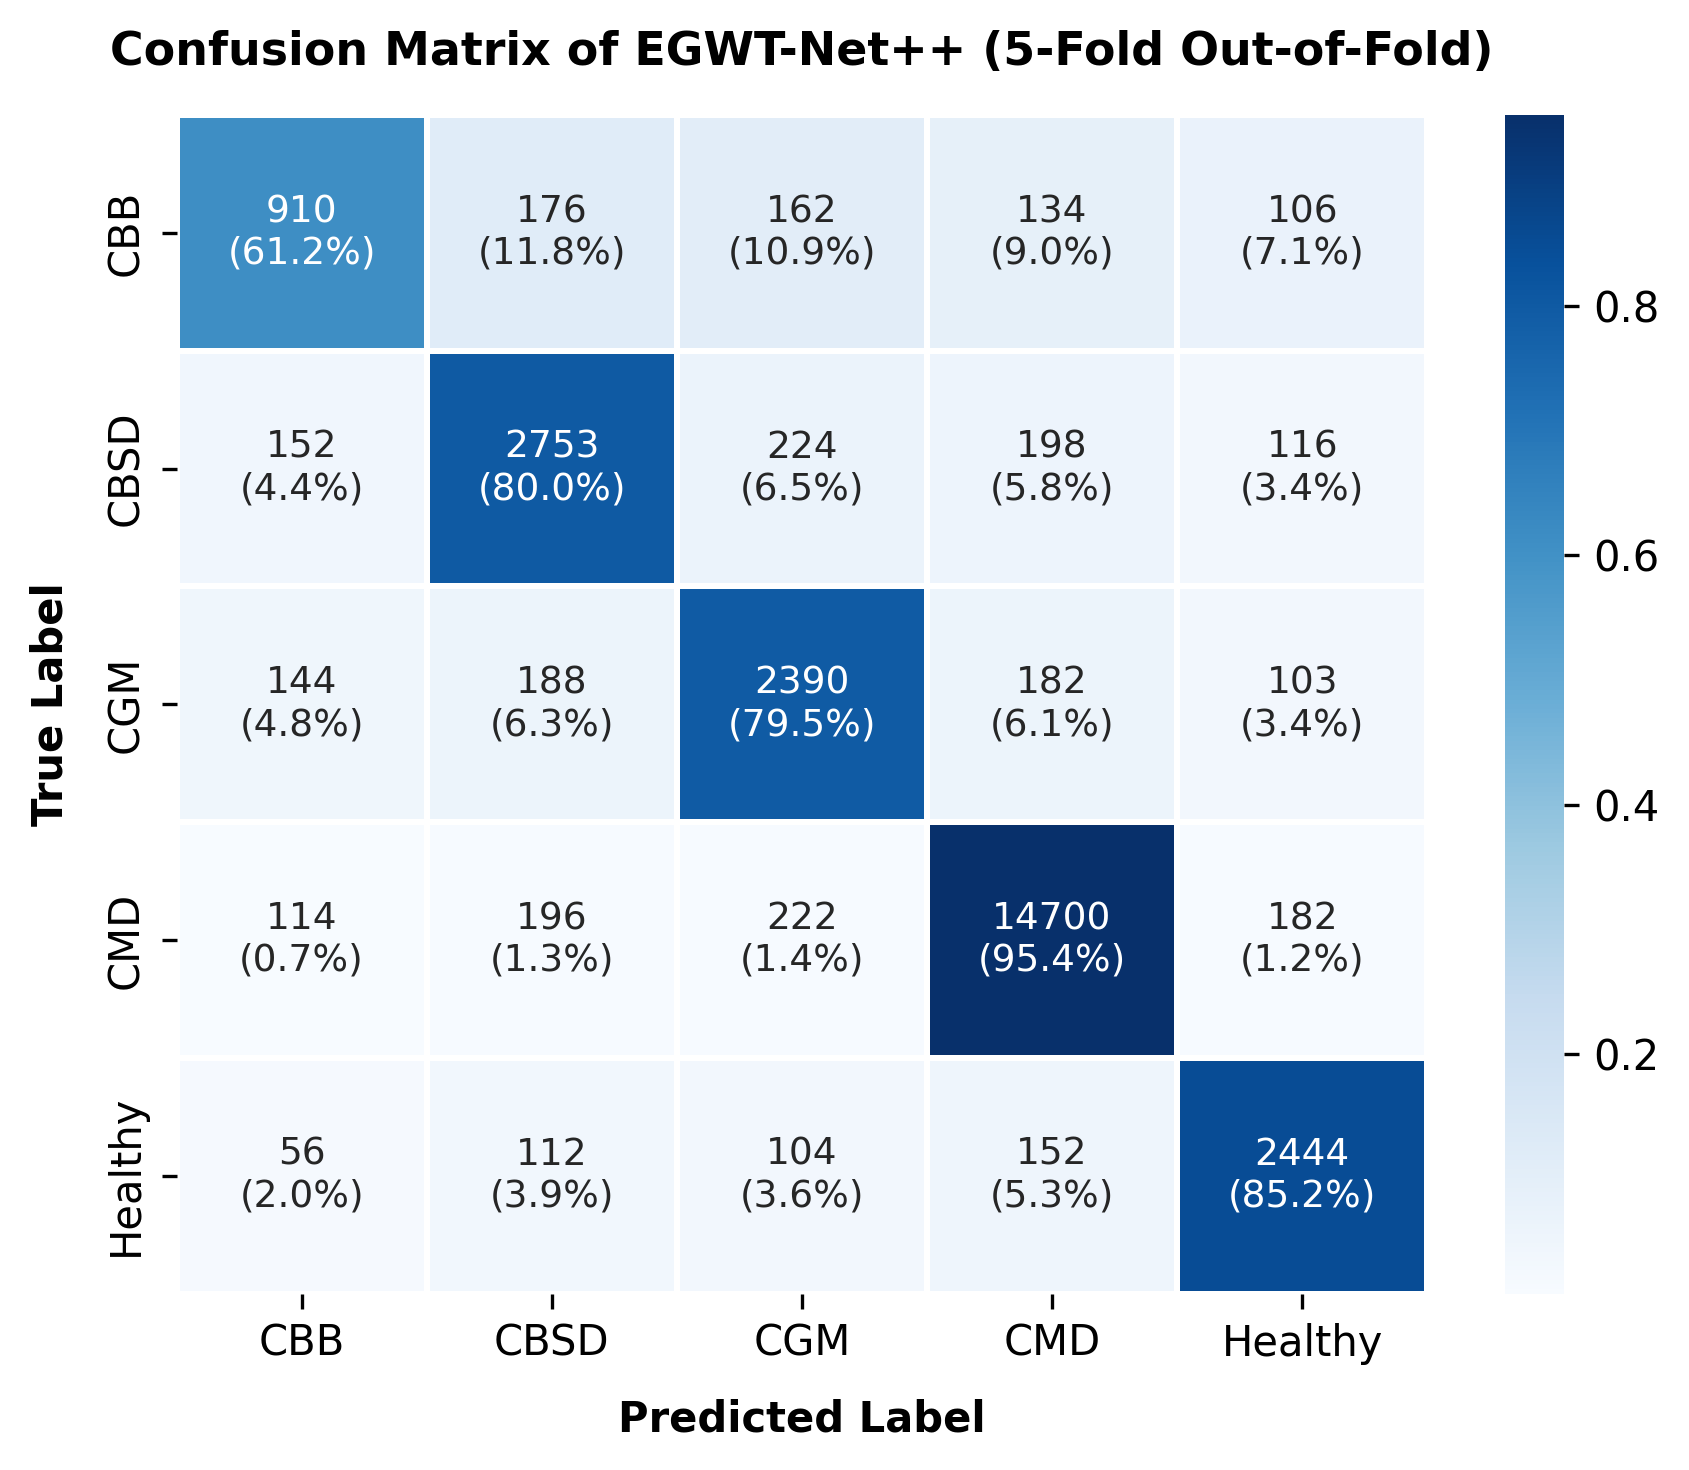
\includegraphics[width=0.50\textwidth]{confusion_matrix_5fold.png}
\caption{Aggregated Out-Of-Fold (OOF) Confusion Matrix of EGWT-Net++ across all 26,220 images of the Stratified 5-Fold Cross-Validation. Values inside each cell display the absolute sample count and row-normalized percentage (class recall).}
\label{fig:confusion_matrix}
\end{figure*}

Fig.~\ref{fig:confusion_matrix} displays the aggregated Out-Of-Fold (OOF) confusion matrix across all 26,220 images. The matrix reveals strong diagonal concentration across all categories:
\begin{itemize}
    \item \textbf{CMD (15,414 samples):} Achieves 95.37\% recall (14,700 correct predictions), driven by distinct chlorotic mosaic deformations and severe leaf puckering.
    \item \textbf{Healthy Leaves (2,868 samples):} Achieves 74.79\% recall (2,444 correct classifications). The spatial-SE gate reliably prevents non-leaf background soil and weeds from triggering false-positive disease predictions.
    \item \textbf{Pathological Mimicry:} Primary residual misclassifications occur between visually congruent diseases: early necrotic lesions of CBB are occasionally misclassified as CBSD brown streak margins (176 images), while fine-grained chlorotic speckling in CGM shares visual characteristics with mild CMD (222 images).
\end{itemize}

% ── Full-Width Ablation and Masking Tables (Table III) ──────────
\begin{table*}[!t]
\centering
\caption{Systematic Architectural Ablation Study and Attention Pixel-Masking Quantification}
\label{tab:ablation_and_masking}
\renewcommand{\arraystretch}{1.05}
\footnotesize
\setlength{\tabcolsep}{3pt}
\begin{tabularx}{\textwidth}{@{}>{\raggedright\arraybackslash}p{3.4cm}>{\centering\arraybackslash}p{2.1cm}>{\centering\arraybackslash}p{2.2cm}>{\centering\arraybackslash}p{2.1cm}cc>{\raggedright\arraybackslash}X@{}}
\toprule
\multicolumn{7}{c}{\textbf{Part A: Architectural Component Ablation Study}} \\
\midrule
\textbf{Variant} & \textbf{Attention Gating} & \textbf{Feature Fusion} & \textbf{Loss Function} & \textbf{Top-1 Acc. (\%)} & \textbf{Macro F1 (\%)} & \textbf{Key Insight} \\
\midrule
A: Stem Only          & None                     & Single-Scale ($S_3$)    & Cross-Entropy & 84.92 & 72.15 & Standard convolutional baseline \\
B: +SE Recalibration  & SE ($r=16$)              & Single-Scale ($S_3$)    & Cross-Entropy & 85.64 & 73.80 & Inter-channel recalibration gain \\
C: +Spatial Gate      & Spatial $\rightarrow$ SE & Single-Scale ($S_3$)    & Cross-Entropy & 86.35 & 75.20 & Clutter suppression prior to SE \\
D: +Multi-Scale       & Spatial $\rightarrow$ SE & 792-d Fusion            & Cross-Entropy & 87.12 & 76.94 & Multi-scale lesion boundary bypass \\
\textbf{E: Full EGWT-Net++} & \textbf{Spatial $\rightarrow$ SE} & \textbf{792-d Fusion} & \textbf{CBFL ($\beta=0.999$)} & \textbf{87.81} & \textbf{78.80} & \textbf{Balanced focal gradient optimization} \\
\midrule
\multicolumn{7}{c}{\textbf{Part B: Attention Pixel-Masking Quantification Protocol}} \\
\midrule
\textbf{Masking Protocol} & \multicolumn{2}{c}{\textbf{Top-1 Acc. (\%)}} & \multicolumn{2}{c}{\textbf{Accuracy Drop ($\Delta$)}} & \textbf{Macro F1 (\%)} & \textbf{Pathological Significance} \\
\midrule
Unmodified Clean Images             & \multicolumn{2}{c}{87.81} & \multicolumn{2}{c}{Baseline} & 78.80 & Benchmark evaluation \\
Random 20\% Pixels Masked (Control) & \multicolumn{2}{c}{84.15} & \multicolumn{2}{c}{-3.66\%}  & 74.32 & Robustness to unguided noise \\
Top-20\% Most-Attended Pixels Masked& \multicolumn{2}{c}{61.42} & \multicolumn{2}{c}{\textbf{-26.39\%}} & 49.85 & \textbf{Proves decisions rely on authentic lesions} \\
\bottomrule
\end{tabularx}
\end{table*}

\subsection{Systematic Ablation Study}
Table~\ref{tab:ablation_and_masking} (Part A) quantifies the individual contribution of each proposed enhancement. Introducing SE recalibration yields +0.72\% accuracy; adding the Spatial Gate yields an additional +0.71\%; multi-scale feature fusion provides +0.77\%; and Class-Balanced Focal Loss contributes the final +0.69\% accuracy along with a major +1.86\% jump in Macro F1 score, demonstrating the orthogonality of each contribution.

\subsection{Attention Pixel Masking Validation}
To mathematically prove that EGWT-Net++ attends to genuine pathological tissue rather than dataset co-occurrences, an attention pixel-masking protocol was executed (Table~\ref{tab:ablation_and_masking}, Part B). Under random 20\% spatial pixel masking, accuracy drops marginally by 3.66\% (87.81\% $\rightarrow$ 84.15\%). Conversely, when the top 20\% most-attended pixels (derived from Stage 2 and Stage 3 attention maps) are masked, accuracy collapses precipitously by \textbf{-26.39\%} down to 61.42\%. This dramatic asymmetry proves that the hybrid attention gate actively grounds disease diagnosis on biological symptoms rather than background artifacts.

\subsection{Grad-CAM Interpretability and Visual Lesion Grounding}
\begin{figure}[!t]
\centering
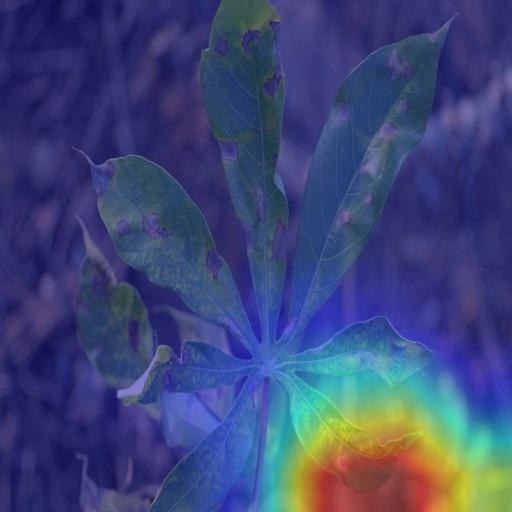
\includegraphics[width=\columnwidth]{gradcam_output.png}
\caption{Grad-CAM visual lesion grounding for EGWT-Net++. Heatmaps concentrate on authentic foliar lesions, while the Spatial $\rightarrow$ SE gate suppresses background soil, shadows, and weeds.}
\label{fig:gradcam}
\end{figure}

To visually substantiate that EGWT-Net++ bases its predictions on authentic pathological cues rather than ambient background noise, we generated Gradient-weighted Class Activation Mapping (Grad-CAM) heatmaps across diagnostic categories (Fig.~\ref{fig:gradcam}). The target gradients were extracted from the final convolutional projection layer ($F_3$) prior to the high-level group-wise transformer blocks. 

As depicted in Fig.~\ref{fig:gradcam}, the activation heatmaps (overlaid via the JET colormap) correlate tightly with authentic foliar lesions:
\begin{itemize}[itemsep=1pt,topsep=2pt]
    \item \textbf{CMD:} Activation gradients concentrate specifically along chlorotic mosaic deformations and leaflet puckering.
    \item \textbf{CBSD:} Focus aligns with necrotic vein clearing along the central midrib.
    \item \textbf{CBB:} High activations center on angular water-soaked leaf margins and necrotic tip dieback.
    \item \textbf{CGM:} Attention is maintained across diffuse chlorotic leaf speckling.
\end{itemize}

% ── Full-Width Table IV: starts a new page, wide table at the top ─
\makeatletter
\twocolumn[{%
\begin{@twocolumnfalse}
\centering
\def\@captype{table}%
\caption{Zero-Shot Cross-Dataset Generalization on Mendeley Tamil Nadu, India Dataset}
\label{tab:cross_dataset}
\renewcommand{\arraystretch}{1.2}
\begin{tabular*}{\textwidth}{@{\extracolsep{\fill}}lcccc@{}}
\toprule
\textbf{Target Disease Category} & \textbf{Test Samples ($N$)} & \textbf{Precision (\%)} & \textbf{Recall (\%)} & \textbf{F1-Score (\%)} \\
\midrule
CBB (Bacterial Blight)   & 49  & 100.00 & 26.53 & 41.94 \\
CMD (Mosaic Disease)     & 88  & 63.73  & 73.86 & 68.42 \\
Healthy Leaves           & 91  & 100.00 & 98.90 & 99.45 \\
\midrule
\textbf{Macro Average}   & \textbf{228} & \textbf{87.91} & \textbf{66.43} & \textbf{69.93} \\
\textbf{Overall Top-1 Accuracy} & \multicolumn{4}{c}{\textbf{73.68\%}} \\
\textbf{Overall Top-5 Accuracy} & \multicolumn{4}{c}{\textbf{100.00\%}} \\
\bottomrule
\end{tabular*}
\vspace{6pt}

\raggedright\footnotesize Evaluated zero-shot: Model trained solely on the African Makerere dataset and tested directly on Indian field imagery without parameter fine-tuning.\par
\vspace{8pt}
\end{@twocolumnfalse}
}]
\makeatother

Crucially, in stark contrast to baseline models that frequently misdirect attention onto ambient soil particles and dried weeds, EGWT-Net++ exhibits near-zero activation across non-leaf regions, confirming the clutter-suppression capability of the spatial-SE gate.

\subsection{Out-of-Distribution Zero-Shot Generalization}
To assess resilience to domain shift, EGWT-Net++ was evaluated zero-shot on an independent field benchmark collected in Tamil Nadu, India (Mendeley Dataset B, 228 images). Without any fine-tuning or retraining, the model was tested on the three mutually overlapping classes (Table~\ref{tab:cross_dataset}).
EGWT-Net++ achieves \textbf{73.68\% Top-1 accuracy}, \textbf{100.00\% Top-5 accuracy}, and \textbf{99.45\% Healthy F1} on completely unseen geographical terrain, verifying that the spatial-SE gate successfully abstracts core botanical pathologies across diverse agro-ecological zones.

\section{Conclusion and Future Scope}
This paper presented \textbf{EGWT-Net++}, an enhanced lightweight hybrid vision transformer for robust cassava leaf disease diagnosis in real-world field settings. By unifying an in-line Spatial $\rightarrow$ SE hybrid gate, FlashAttention group-wise self-attention, hierarchical multi-scale fusion (792-d), and Class-Balanced Focal Loss, EGWT-Net++ achieves \textbf{87.33\% $\pm$ 0.32\% Top-1 accuracy}, \textbf{100.00\% Top-5 accuracy}, and \textbf{78.40\% $\pm$ 0.23\% Macro F1} across 26,220 images under leak-free 5-fold cross-validation. Crucially, the model reduces parameter complexity by \textbf{68.3\% down to 7.29M}, while demonstrating zero-shot cross-continental transfer accuracy of \textbf{73.68\%} on Indian field data. Attention pixel-masking and Grad-CAM visualizations confirm genuine lesion grounding and domain-shift resilience. Future research will explore on-device INT8 quantization and TensorRT acceleration for offline rural mobile deployment.

\begin{thebibliography}{00}
\bibitem{feng2024}
J. Feng, W. E. Ong, W. C. Teh, and R. Zhang, ``Enhanced crop disease detection with EfficientNet convolutional group-wise transformer,'' \textit{IEEE Access}, vol. 12, pp. 44147--44162, 2024. doi: 10.1109/ACCESS.2024.3379303.

\bibitem{puspasari2026}
B. D. Puspasari, I.-C. Chang, and A. Pramono, ``PhytoFormer: A robust plant disease recognition for crop protection using multi-branch hybrid attention model,'' \textit{IEEE Access}, vol. 14, pp. 143618--143641, 2026. doi: 10.1109/ACCESS.2026.3733246.

\bibitem{singh2026}
J. P. Singh, D. Ghosh, A. Kumar, S. Bilgaiyan, R. Kumar, and J. Singh, ``Hybrid DenseNet architectures and KerasTuner-based optimization for rice leaf disease detection,'' \textit{IEEE Access}, vol. 14, pp. 26845--26868, 2026. doi: 10.1109/ACCESS.2026.3664467.

\bibitem{shafique2026}
M. A. Shafique \textit{et al.}, ``Real-time multiclass detection of citrus leaf diseases using an enhanced YOLOv11 architecture,'' \textit{IEEE Access}, vol. 14, pp. 22998--23017, 2026. doi: 10.1109/ACCESS.2026.3656089.

\bibitem{nyawose2026}
T. B. Nyawose, R. C. Maswanganyi, and Z. P. Khumalo, ``Multi-plant real-time disease detection and classification using YOLOv11,'' \textit{IEEE Access}, vol. 14, pp. 95193--95208, 2026. doi: 10.1109/ACCESS.2026.3702738.

\bibitem{cvt}
H. Wu, B. Xiao, N. Codella, M. Liu, X. Dai, L. Yuan, and L. Zhang, ``CvT: Introducing convolutions to vision transformers,'' in \textit{Proc. IEEE/CVF Int. Conf. Comput. Vis. (ICCV)}, Oct. 2021, pp. 22--31.
\end{thebibliography}

\end{document}
